
\subsection{UniSiegen dataset}

This dataset is made available in 2014 by the University of Siegen, Germany.
It was constructed by dr. D. Zukic \cite{Zukic2014} as part of his PhD project.

\marginpar{
        % This file was created by tikzplotlib v0.9.8.
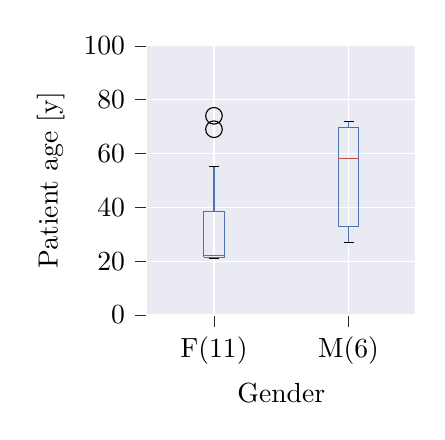
\begin{tikzpicture}

\definecolor{color0}{rgb}{0.917647058823529,0.917647058823529,0.949019607843137}
\definecolor{color1}{rgb}{0.298039215686275,0.447058823529412,0.690196078431373}
\definecolor{color2}{rgb}{0.768627450980392,0.305882352941176,0.32156862745098}

\begin{axis}[
axis background/.style={fill=color0},
axis line style={white},
height=5cm,
tick align=outside,
tick pos=left,
width=5cm,
x grid style={white},
xlabel={Gender},
xmajorgrids,
xmin=0.5, xmax=2.5,
xtick style={color=white!15!black},
xtick={1,2},
xticklabels={F(11),M(6)},
y grid style={white},
ylabel={Patient age [y]},
ymajorgrids,
ymin=0, ymax=100,
ytick style={color=white!15!black}
]
\addplot [color1, opacity=1]
table {%
0.925 21.5
1.075 21.5
1.075 38.5
0.925 38.5
0.925 21.5
};
\addplot [color1, opacity=1]
table {%
1 21.5
1 21
};
\addplot [color1, opacity=1]
table {%
1 38.5
1 55
};
\addplot [black, opacity=1]
table {%
0.9625 21
1.0375 21
};
\addplot [black, opacity=1]
table {%
0.9625 55
1.0375 55
};
\addplot [black, mark=o, mark size=3, mark options={solid,fill opacity=0}, only marks]
table {%
1 74
1 69
};
\addplot [color1, opacity=1]
table {%
1.925 33
2.075 33
2.075 69.5
1.925 69.5
1.925 33
};
\addplot [color1, opacity=1]
table {%
2 33
2 27
};
\addplot [color1, opacity=1]
table {%
2 69.5
2 72
};
\addplot [black, opacity=1]
table {%
1.9625 27
2.0375 27
};
\addplot [black, opacity=1]
table {%
1.9625 72
2.0375 72
};
\addplot [color2, opacity=1]
table {%
0.925 22
1.075 22
};
\addplot [color2, opacity=1]
table {%
1.925 58
2.075 58
};
\end{axis}

\end{tikzpicture}

        \captionof{figure}{USiegen patients age distribution}
        \label{fig:USiegen_Age}
    }

This dataset contains 26 \acrshort{mri} scans of 17 different patients. 
The fact that scans of the same patient are correlated will be taken into account 

\subsubsection{Original Objective of the Dataset}

This dataset was collected from several hospitals (Sarajevo, Marburg, Brisbane, Schwabach, Bad Wildungen \& Prague). The MRI scanner settings were varied between the scans (T1, T2, TIRM).
The PhD project objective was to build a segmentation model to automate the segmentation of the lumbar vertebrae in the \acrshort{mri} scans to facilitate the diagnosis of several spine pathologies 
such as scoliosis, spondylolisthesis \footnote{Spondylolisthesis is the displacement of one spinal vertebra compared to another.} and vertebral fractures.
The final model developed by dr. D. Zukic consisted of a Viola-Jones detector for detection and vertebral body size approximation.
The average Dice score compared to the manual reference was reported to be 79.3\%.

\subsubsection{Patient statistics}

In \cite{Zukic2014}, it is not fully made clear which scans are taken from the same patient.
It is made clear however that the 26 scans were not obtained from 26 patients.
I inferred the information from the naming of the scans and the provided gender en age information\footnote{
    Wrongfully assuming two scans come from the same patient does not cause data leakage in the used approach.
}.

Figure \ref{fig:USiegen_Age} illustrates that the USiegen dataset contains almost double the amount of female patients compared to male patients.
These patients are relatively young compared to the patients in the \textit{xVertSeg} dataset.

Only three of the patients in this dataset were categorized as having no spinal pathologies.

\subsubsection{Technical information}

Several \acrlong{mri} techniques were used to obtain the dataset: T1, T2 \& TIRM.
I do not take into account this factor in the model development.

\begin{SCfigure}[][htb]
    \centering
    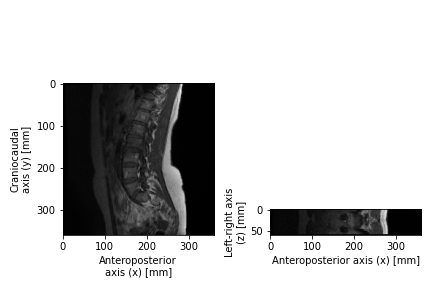
\includegraphics[width=.95\textwidth]{automated_graphs/USiegen_Aka3.png}
    \caption{USiegen dataset scan \textit{Aka3}. \label{fig:USiegen_Aka3}}
\end{SCfigure}

The original scans in the \textit{USiegen} dataset were cropped in the \textit{left-right} direction. 
Although the scan resolution is relatively high in the Sagittal planes, the slice spacing along the left-right axis is coarser (see figure \ref{fig:AllDataset_dims}).  